% Foliensatz: "AFu-Kurs nach DJ4UF" von DK0TU, Amateurfunkgruppe der TU Berlin
% Lizenz: CC BY-NC-SA 3.0 de (http://creativecommons.org/licenses/by-nc-sa/3.0/de/)
% Autoren: Felix Baum <baum@campus.tu-berlin.de>
% Korrekturen: Lars Weiler <dc4lw@darc.de>

\documentclass[aspectratio=169]{beamer}

\usepackage[ngerman]{babel} % deutsche Worttrennung etc.
\usepackage[utf8]{inputenc} % UTF8 Text

\usepackage[super, comma, numbers, square, sort]{natbib}

\usepackage{hyperref}       % Hyperref Package für bessere Referenzen (todo)
\hypersetup{
	colorlinks=false,       %   false: boxed links; true: colored links
    %linkcolor=white,       %   color of internal links (change box color with linkbordercolor)
    citecolor=red,          %   color of links to bibliography
    filecolor=white,        %   color of file links
    urlcolor=blue           %   color of external links
}

\usepackage{multirow}
\usepackage{wasysym}  % Math Symbols like \permil
%\usepackage{colortbl}
%\usepackage{subscript}
%\usepackage{caption}
%\usepackage{setspace}
%\usepackage{xcolor}        % benutze CodeListe

% Footnote
%\usepackage{hanging}
%
%\setbeamertemplate{footnote}{%
%  \hangpara{2em}{1}%
%  \makebox[2em][l]{\insertfootnotemark}\footnotesize\insertfootnotetext\par%
%}


%\usepackage{pgf}
%\usepackage{tikz}
%\usetikzlibrary{arrows,automata}
%\usetikzlibrary{positioning}
%
%\tikzset{
%    state/.style={
%           rectangle,
%           rounded corners,
%           draw=black, very thick,
%           minimum height=2em,
%           minimum width=2pt,
%           inner sep=2pt,
%           text centered,
%           },
%}

%\usepackage{listings}
%\lstset{basicstyle=\small, numberstyle=\tiny, extendedchars=true, numbers=left, numbersep=5pt}
%\lstset{showtabs=false, showspaces=false, showstringspaces=false}
%%\lstset{backgroundcolor=\color{white!75!lightgray}, , frame=single}
%%\lstset{backgroundcolor=\color{white}}
%%\lstset{backgroundcolor=none}
%\lstset{keywordstyle=\color{blue!50!gray},  identifierstyle=\color{black}}
%\lstset{commentstyle=\color{green!50!gray}, stringstyle=\color{red!50!gray}}
%\lstset{language=C, fontadjust=true, tabsize=2, breaklines=true}
%\lstset{backgroundcolor=\color{white!75!lightgray}, caption=\lstname, frame=single}
%\lstset{emphstyle=\color{black}\fbox}
%
%% Keine "Listing:"-Caption
%\captionsetup{labelformat=empty,labelsep=none}
%
%% für mathematische Umgebungen
%\usepackage{amsmath,amsfonts,amssymb}
%
%\lstdefinestyle{Bash}{
%language=Bash,
%frame=single,
%rulecolor=\color{black},
%backgroundcolor=\color{gray!50},
%keywordstyle=\color{black},
%identifierstyle=,
%commentstyle=\color{black},
%stringstyle=\color{magenta!65!white},
%showstringspaces=false,
%basicstyle=\footnotesize\ttfamily\color{black},
%numbers=none,
%breaklines=true,
%captionpos=b
%}

%\usepackage{listings}
%
%\lstdefinestyle{basic}{
%    captionpos=t,%
%    basicstyle=\footnotesize\ttfamily,%
%    numberstyle=\tiny,%
%    numbers=left,%
%    stepnumber=1,%
%    frame=single,%
%    showspaces=false,%
%    showstringspaces=false,%
%    showtabs=false,%
%    %
%    keywordstyle=\color{blue},%
%    identifierstyle=,%
%    commentstyle=\color{gray},%
%    stringstyle=\color{magenta}%
%}



% fließende Boxen haben keinen Abstand
%\fboxsep0mm

% inkludiere Creative Commons Helper
%%%%%%%%%%%%%%%%%%%%%%%%%%%%%%%%%%%%%%%%%%%%%%%%%%%%%%%%%%%%%%%%
%% ccBeamer 0.1, 2007-07-02                                   %%
%% Written by Sebastian Pipping <webmaster@hartwork.org>      %%
%% ---------------------------------------------------------- %%
%% Licensed under Creative Commons Attribution-ShareAlike 3.0 %%
%% http://creativecommons.org/licenses/by-sa/3.0/             %%
%%%%%%%%%%%%%%%%%%%%%%%%%%%%%%%%%%%%%%%%%%%%%%%%%%%%%%%%%%%%%%%%


%% Images
\newcommand{\CcImageBy}[1]{%
	
\includegraphics[scale=#1]{texdata/creative_commons/cc_by_30.pdf}%
}
\newcommand{\CcImageCc}[1]{%
	
\includegraphics[scale=#1]{texdata/creative_commons/cc_cc_30.pdf}%
}
\newcommand{\CcImageDevNations}[1]{%
	
\includegraphics[scale=#1]{texdata/creative_commons/cc_dev_nations_30.pdf}%
}
\newcommand{\CcImageNc}[1]{%
	
\includegraphics[scale=#1]{texdata/creative_commons/cc_nc_30.pdf}%
}
\newcommand{\CcImageNd}[1]{%
	
\includegraphics[scale=#1]{texdata/creative_commons/cc_nd_30.pdf}%
}
\newcommand{\CcImagePd}[1]{%
	
\includegraphics[scale=#1]{texdata/creative_commons/cc_pd_30.pdf}%
}
\newcommand{\CcImageSa}[1]{%
	
\includegraphics[scale=#1]{texdata/creative_commons/cc_sa_30.pdf}%
}
\newcommand{\CcImageSampling}[1]{%
	
\includegraphics[scale=#1]{texdata/creative_commons/cc_sampling_30.pdf}%
}
\newcommand{\CcImageSamplingPlus}[1]{%
	
\includegraphics[scale=#1]{texdata/creative_commons/cc_sampling_plus_30.pdf}%
}


%% Groups
\newcommand{\CcGroupBy}[2]{% zoom, gap
	\CcImageCc{#1}\hspace*{#2}\CcImageBy{#1}%
}
\newcommand{\CcGroupByNc}[2]{% zoom, gap
	\CcImageCc{#1}\hspace*{#2}\CcImageBy{#1}\hspace*{#2}\CcImageNc{#1}%
}
\newcommand{\CcGroupByNcNd}[2]{% zoom, gap
	\CcImageCc{#1}\hspace*{#2}\CcImageBy{#1}\hspace*{#2}\CcImageNc{#1}\hspace*{#2}\CcImageNd{#1}%
}
\newcommand{\CcGroupByNcSa}[2]{% zoom, gap
	\CcImageCc{#1}\hspace*{#2}\CcImageBy{#1}\hspace*{#2}\CcImageNc{#1}\hspace*{#2}\CcImageSa{#1}%
}
\newcommand{\CcGroupByNd}[2]{% zoom, gap
	\CcImageCc{#1}\hspace*{#2}\CcImageBy{#1}\hspace*{#2}\CcImageNd{#1}%
}
\newcommand{\CcGroupBySa}[2]{% zoom, gap
	\CcImageCc{#1}\hspace*{#2}\CcImageBy{#1}\hspace*{#2}\CcImageSa{#1}%
}
\newcommand{\CcGroupDevNations}[2]{% zoom, gap
	\CcImageCc{#1}\hspace*{#2}\CcImageDevNations{#1}%
}
\newcommand{\CcGroupNcSampling}[2]{% zoom, gap
	\CcImageCc{#1}\hspace*{#2}\CcImageNc{#1}\hspace*{#2}\CcImageSampling{#1}%
}
\newcommand{\CcGroupPd}[1]{% zoom
	\CcImagePd{#1}%
}
\newcommand{\CcGroupSampling}[1]{% zoom
	\CcImageSampling{#1}%
}
\newcommand{\CcGroupSamplingPlus}[1]{% zoom
	\CcImageSamplingPlus{#1}%
}


%% Text
\newcommand{\CcLongnameBy}{Attribution}
\newcommand{\CcLongnameByNc}{Attribution-NonCommercial}
\newcommand{\CcLongnameByNcNd}{Attribution-NoDerivs}
\newcommand{\CcLongnameByNcSa}{Attribution-NonCommercial-ShareAlike}
\newcommand{\CcLongnameByNd}{Attribution-NoDerivs}
\newcommand{\CcLongnameBySa}{Attribution-ShareAlike}

\newcommand{\CcNote}[1]{% longname
	This work is licensed under the \textit{Creative Commons #1 3.0 License}.%
}


% generelles Thema auswählen
\usetheme{Goettingen} %Berlin spart ohne Sidebar allerdings angenehm Platz
% AnnArbor | Antibes | Bergen | Berkeley | Berlin | Boadilla | boxes | CambridgeUS | Copenhagen | Darmstadt | default | Dresden | Frankfurt | Goettingen | Hannover | Ilmenau | JuanLesPins | Luebeck | Madrid | Malmoe | Marburg | Montpellier | PaloAlto | Pittsburgh | Rochester | Singapore | Szeged | Warsaw

% Farben wählen
\usecolortheme{beetle}
% beaver | beetle | crane | default | dolphin | dove | fly | lily | orchid | rose | seagull | seahorse | sidebartab | structure | whale | wolverine

% Setze alle Farben auf Grau und Weiß
%\definecolor{craneorange}{RGB}{64,64,64}
%\definecolor{craneblue}{RGB}{255,255,255}

% Schriftart wählen
\usefonttheme{default}
% default | professionalfonts | serif | structurebold | structureitalicserif | structuresmallcapsserif

% Innere Themen(Kopf-, Fuß-, Sidebar usw)
%\useinnertheme{default}
\useinnertheme{circles}
% default | inmargin | rectangles | rounded | circles

% Äußere Themen (Anordnung der inneren, grenzen der Folien etc.)
\useoutertheme{infolines}
% default | infolines | miniframes | shadow | sidebar | smoothbars | smoothtree | split | tree

% Deaktiviere Navigations-Symbole ({} -> leer)
\setbeamertemplate{navigation symbols}{}
%\setbeamertemplate{navigation symbols}{\large \ifnum \insertframenumber <10 0\fi\insertframenumber/\inserttotalframenumber\vspace*{0.2ex}}

% Zeige ein Hintergrundbild
\setbeamertemplate{background canvas}{
        \hspace*{-2.0cm}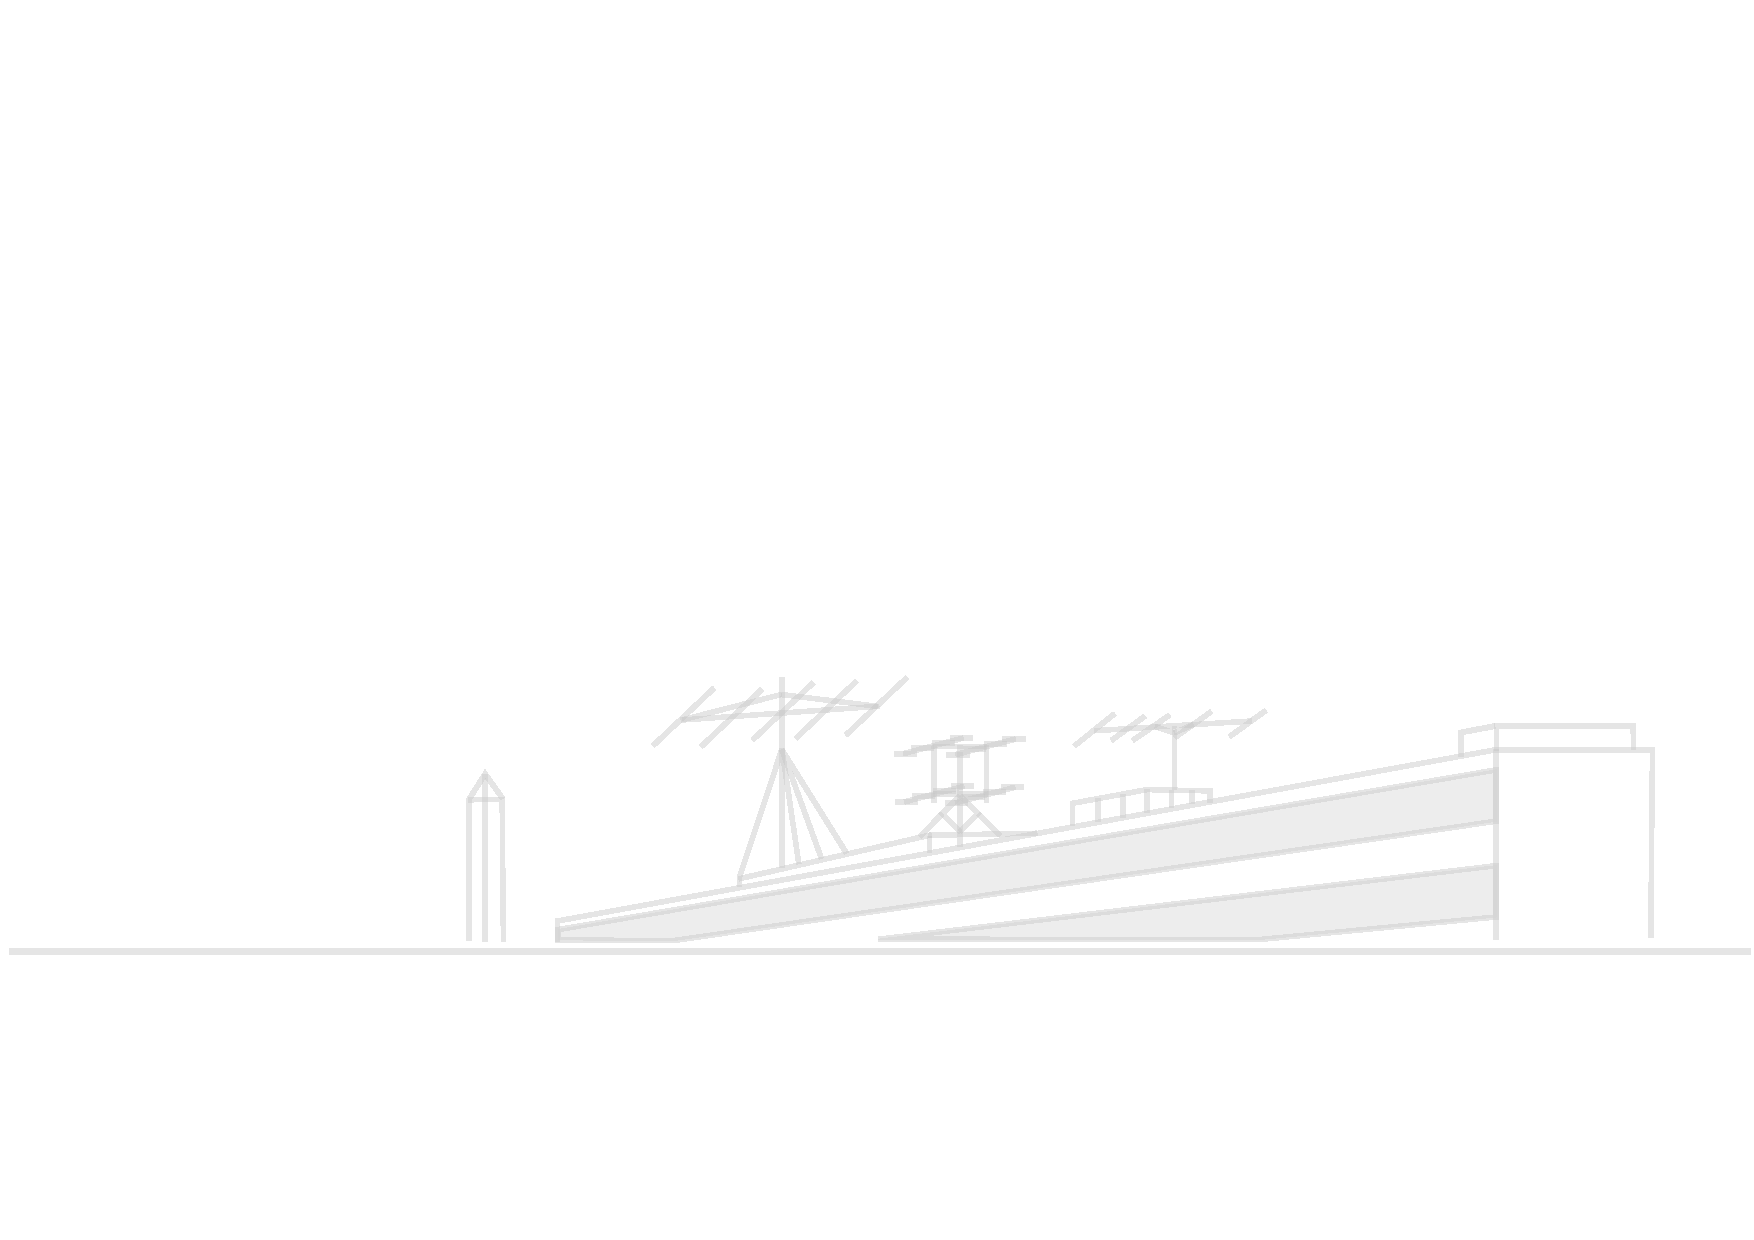
\includegraphics[width=17.8cm]{texdata/dk0tu_rooftop_background.pdf}
}

% Foliennummer einfügen
\setbeamertemplate{footline}[frame number]
%\setbeamertemplate{footline}{}

% Ändere das Zeichen vor jedem item
%\setbeamertemplate{itemize item}{\color{craneorange}$\blacktriangleright$}
%\setbeamertemplate{itemize subitem}{\color{craneorange}$\triangleright$}
%\setbeamertemplate{itemize subsubitem}{\color{craneorange}$\blacktriangleright$}

% Ändert die Blöcke 
\setbeamertemplate{blocks}[rounded][shadow=true]
% default | rounded [shadow=true|false]

%
% Eigene Kommandos
%

% Hack to get natbib and beamer working together. "The beamer user guide suggests
% that only the manual bibliography entry approach is supported"
% on some system it works out of the box, sometimes you need the hack :-(
% so check it --dl7bst
\ifdefined\newblock
    \relax
\else
    \newcommand{\newblock}{}
\fi

% \includedia command to generate png out of a dia file
% NEEDS installed dia and pdflatex option --shell-escape
\newcommand{\includedia}[1]{
    \immediate\write18{/usr/bin/dia #1.dia -e #1_diatmp.png -t png}
}

% RICHIG GROSSER FONT!
\newfont{\bigfont}{cmr10 at 144pt}
\newfont{\smallfont}{cmr10 at 8pt}

% Römische Ziffern
\makeatletter
\newcommand{\rmnum}[1]{\romannumeral #1}
\newcommand{\Rmnum}[1]{\expandafter\@slowromancap\romannumeral #1@}
\makeatother

% Schwarze Überschrift
%\setbeamercolor{frametitle}{fg=black}
%\setbeamercolor{title}{fg=black}

% Item- und Box-Farben
\definecolor{deepBlue}{HTML}{000066}
\setbeamercolor{itemize item}{fg=deepBlue}
\setbeamercolor{itemize subitem}{fg=deepBlue}
\setbeamercolor{description item}{fg=deepBlue}
\setbeamercolor{block title}{fg=deepBlue!100, bg=blue!15}
\setbeamercolor{block body}{fg=black, bg=blue!5}
\setbeamercolor{block title alerted}{fg=deepBlue, bg=red!75}
\setbeamercolor{block body alerted}{fg=black, bg=red!15}
\setbeamercolor*{block title example}{fg=blue!50, bg=blue!10}
\setbeamercolor*{block body example}{fg= blue, bg=blue!5}

%\setbeamercolor{section in head/foot}{parent=palette primary}
%\setbeamercolor{subsection in head/foot}{parent=palette secondary}
%\setbeamercolor{sidebar}{fg=darkblue,bg=yellow!90!orange}
%\setbeamercolor{title in sidebar}{fg=darkblue}
%\setbeamercolor{author in sidebar}{fg=darkblue}
%\setbeamercolor{section in sidebar}{fg=darkblue!10!black}
%\setbeamercolor{subsection in sidebar}{fg=darkblue!50!black}

% Titlepage Infos
\title{AFu-Kurs nach DJ4UF}
\author[DKØTU]{DKØTU\\ \footnotesize{Amateurfunkgruppe der TU Berlin}}
\institute[DKØTU]{\url{http://www.dk0tu.de} }

% PDF-Eigenschaften
\subject{DK0TU-Amateurfunkkurs nach DJ4UF}
\keywords{Amateurfunk Kurs HAM Radio Course CC-BY-NC-SA OpenSource TU Berlin DK0TU}

\subtitle{Technik 11: \\
  Antennentechnik \\[2em]}
\date{Stand 18.09.2017}
 \begin{document}

\begin{frame}
    \titlepage
    \vfill
    \begin{center}
        \ccbyncsaeu\\
        {\tiny This work is licensed under the \em{Creative Commons Attribution-NonCommercial-ShareAlike 3.0 License}.}\\[0.5ex]
         \tiny Amateurfunkgruppe der Technische Universität Berlin (AfuTUB), DKØTU
         %\includegraphics[scale=0.5]{img/DK0TU_Logo.pdf}
    \end{center}
\end{frame}


\section*{Einleitung}

\begin{frame}
  \frametitle{Antenne}
  \begin{center}
    \begin{figure}
      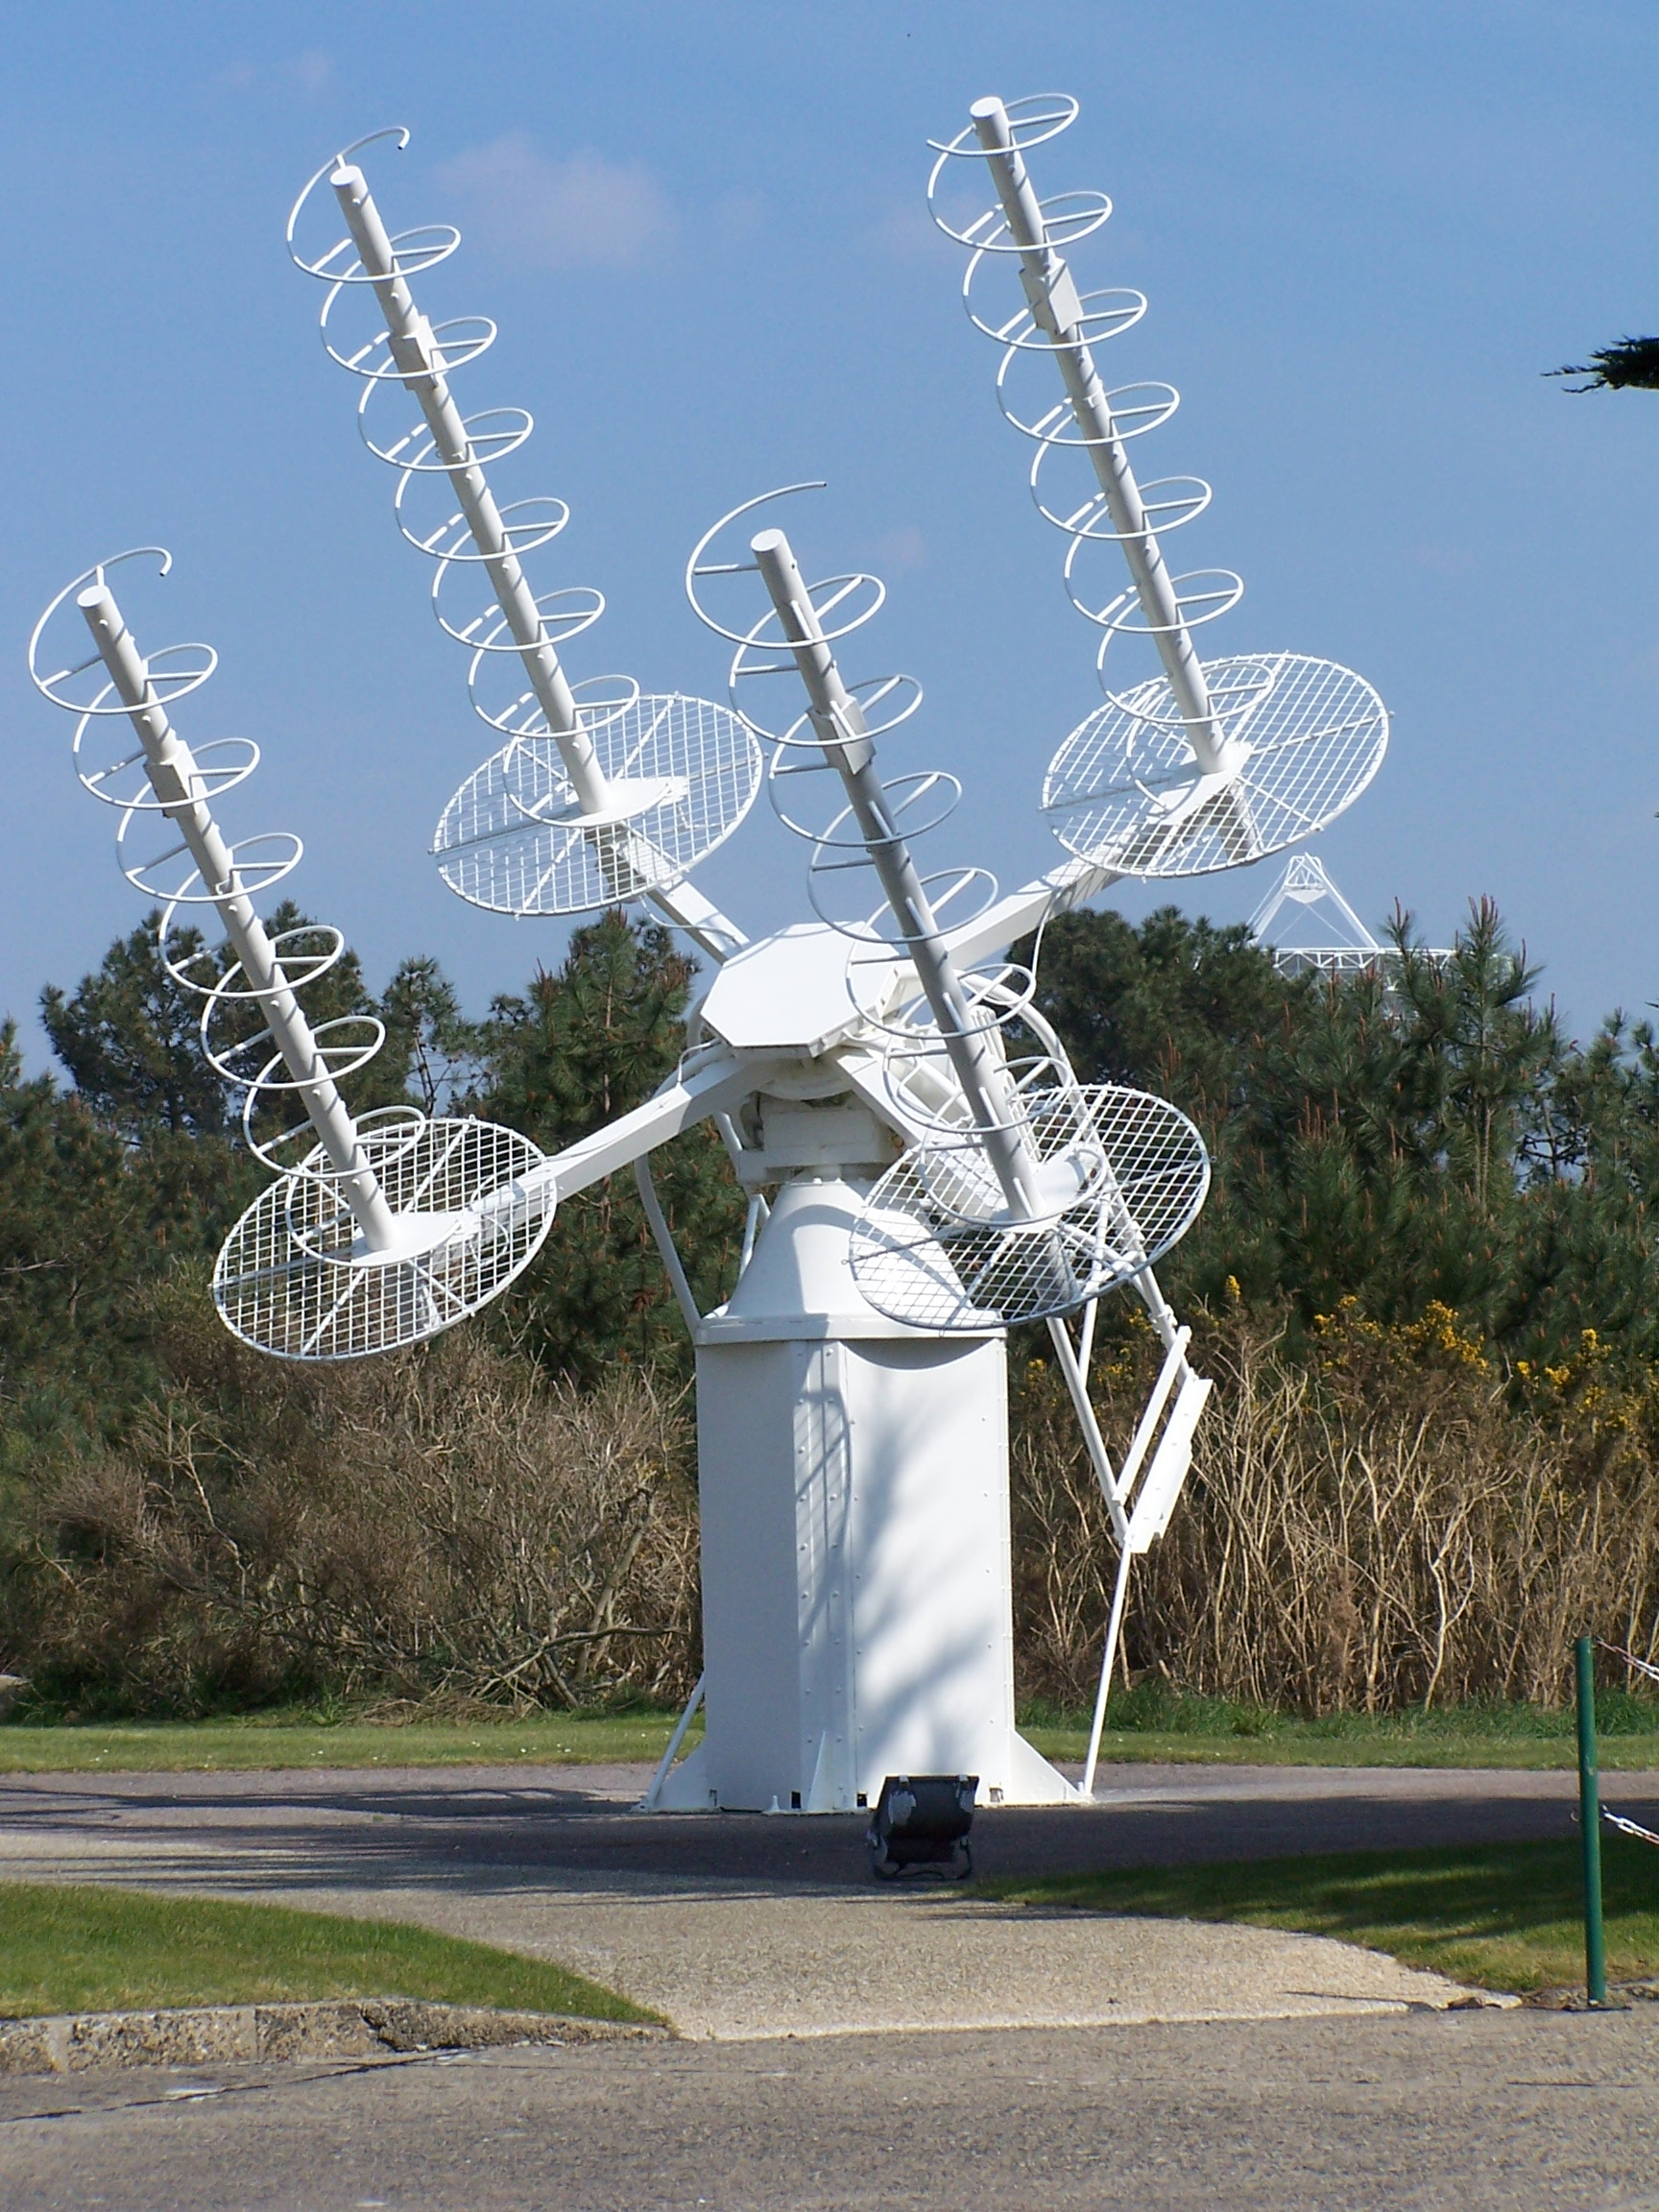
\includegraphics[width=.5\textwidth,height=.7\textheight,keepaspectratio]{e11/Traqueur_acquisition.JPG}
      \attribcaption{Satellite tracking-aquisition antenna}{Kingbastard}{https://commons.wikimedia.org/wiki/File:Traqueur_acquisition.JPG}{\ccbysa}
    \end{figure}
  \end{center}
\end{frame}

\begin{frame}
  \frametitle{Einleitung}
  \begin{minipage}{0.49\textwidth}
    \begin{figure}
      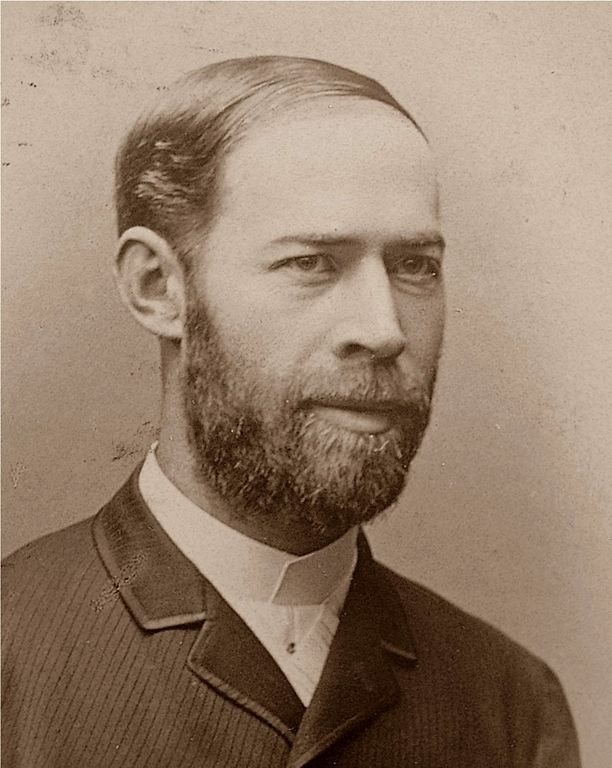
\includegraphics[width=0.9\textwidth,height=.8\textheight,keepaspectratio]{e11/HEINRICH_HERTZ.jpg}
      \attribcaption{Heinrich Hertz}{}{https://commons.wikimedia.org/wiki/File:HEINRICH_HERTZ.JPG}{\ccpd}
    \end{figure}
  \end{minipage}
  \begin{minipage}{0.49\textwidth}
    \begin{itemize}
      \item Heinrich Hertz (1857-1894)
      \item Nachweis elektromagnetischer Wellen 1888
      \item Hertz'sche Dipol
    \end{itemize}
  \end{minipage}
\end{frame}

\begin{frame}
  \frametitle{Schwingkreis}
  \begin{center} \huge
    $$f = \frac{1}{2  \pi \cdot \sqrt{LC}}$$
    \begin{figure}
      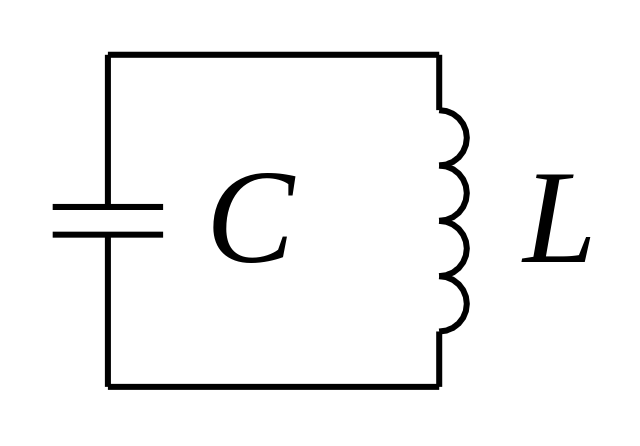
\includegraphics[width=.5\textwidth,height=.3\textheight,keepaspectratio]{e11/Schwingkreis.png}
      \caption{Schwingkreis}
    \end{figure}
  \end{center}
\end{frame}

\begin{frame}
  \frametitle{Dipol}
  \begin{center}
    \begin{figure}
      \begin{figure}
        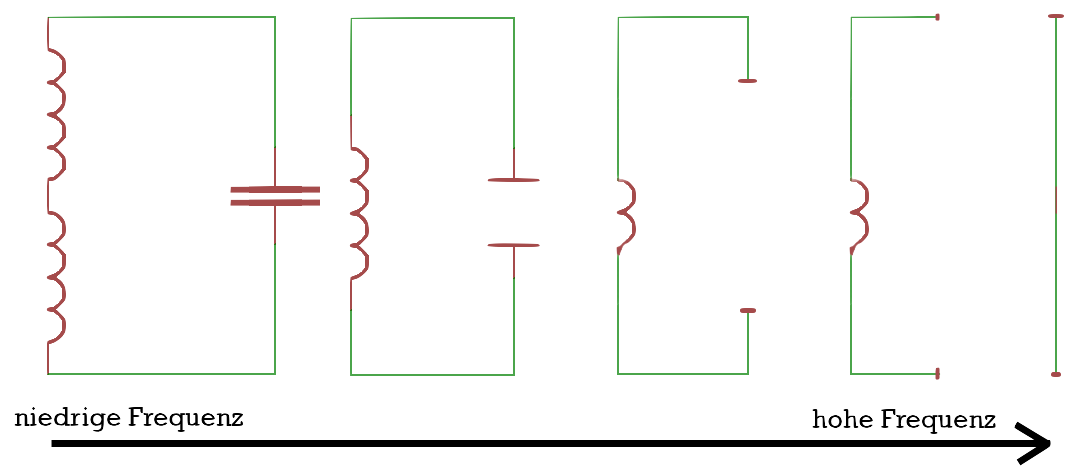
\includegraphics[width=1\textwidth,height=.8\textheight,keepaspectratio]{e11/dipol_entstehung.png}
        \caption{Dipolentstehung}
      \end{figure}
    \end{figure}
  \end{center}
\end{frame}

\begin{frame}
  \frametitle{E- und H-Feld}
  \begin{center}
    \begin{figure}
      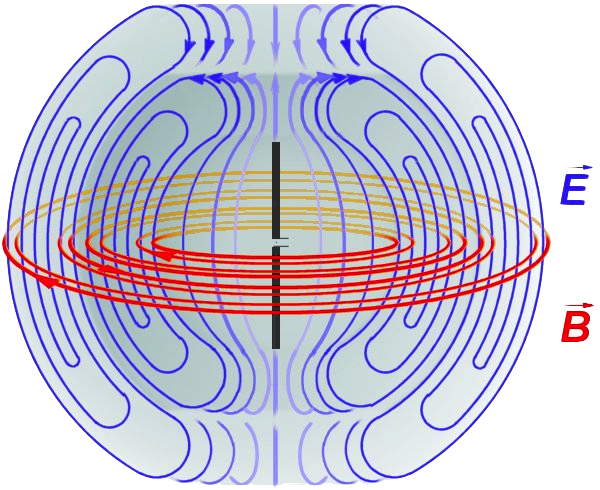
\includegraphics[width=0.85\textwidth,height=.75\textheight,keepaspectratio]{e11/Felder_um_Dipol.png}
      \attribcaption{Felder um Dipol}{Averse}{https://commons.wikimedia.org/wiki/File:Felder_um_Dipol.jpg}{\ccbysa}
    \end{figure}
  \end{center}
\end{frame}

\begin{frame}
  \frametitle{Allgemeines}
  \begin{itemize}
    \item Jeder ungeschirmte Draht ist eine Antenne
    \item Grundsätzlich sind Sende- und Empfangsantennen ähnlich
    \item Alle guten Kurzwellen Sendeantennen sind auch gute Empfangsantennen
    \item Der Antennengewinn bei Sendeantennen gilt ebenso für den Empfang
    \item Umgekehrt nicht immer der Fall (z.B. Ferritantenne)
  \end{itemize}
\end{frame}

\section*{Dipol}

\begin{frame}
  \frametitle{Dipol}
  \begin{center}
    \begin{figure}
      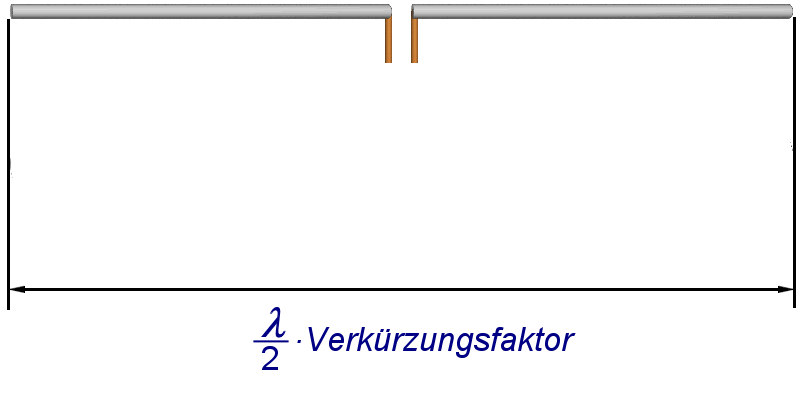
\includegraphics[width=1\textwidth,height=.75\textheight,keepaspectratio]{e11/Faltdipol.png}
      \attribcaption{Faltdipol}{Averse}{https://commons.wikimedia.org/wiki/File:Faltdipol.png}{\ccbysa}
    \end{figure}
  \end{center}
\end{frame}


\begin{frame}
  \frametitle{Wellenlänge}
  \begin{center} \huge
    $$\lambda = \frac{c}{f}$$
    mit $c = 299\,792\,458 \frac{m}{s}$
  \end{center}
\end{frame}

\begin{frame}
  \frametitle{Wellenlänge einfacher}
  \begin{center} \huge
    $$\lambda [m] \approx \frac{300}{f[MHz]}$$
  \end{center}
\end{frame}

%\begin{frame}

%    \frametitle{$\lambda / 2$ Dipol berechnen}
%    \begin{center}
% \begin{itemize} \Large
%  \item Theoretische Strahlerlänge eines $\lambda / 2$ Dipols für 7MHz berechnen
%  \item $\lambda[m] = \frac{300}{f[MHz]}$
%    \end{itemize}
%    \end{center}
%\end{frame}

\begin{frame}
  \frametitle{Verkürzungsfaktor beachten}
  \begin{center}
    \begin{itemize} \Large
      \item Innerhalb von Feststoffen breiten sich EM-Wellen nicht mit Lichtgeschwindigkeit aus
      \item Deshalb: $\lambda[m] = \frac{300}{f[MHz]} \cdot $ Verkürzungsfaktor
      \item Beispiele:
      \begin{itemize}
        \item Kupfer 0,95
        \item RG-213 Koaxialkabel 0,66
        \item Glasfaser 0,67
      \end{itemize}
    \end{itemize}
  \end{center}
\end{frame}

\begin{frame}
  \frametitle{Fertig?}
  \begin{center}
    \begin{figure}
      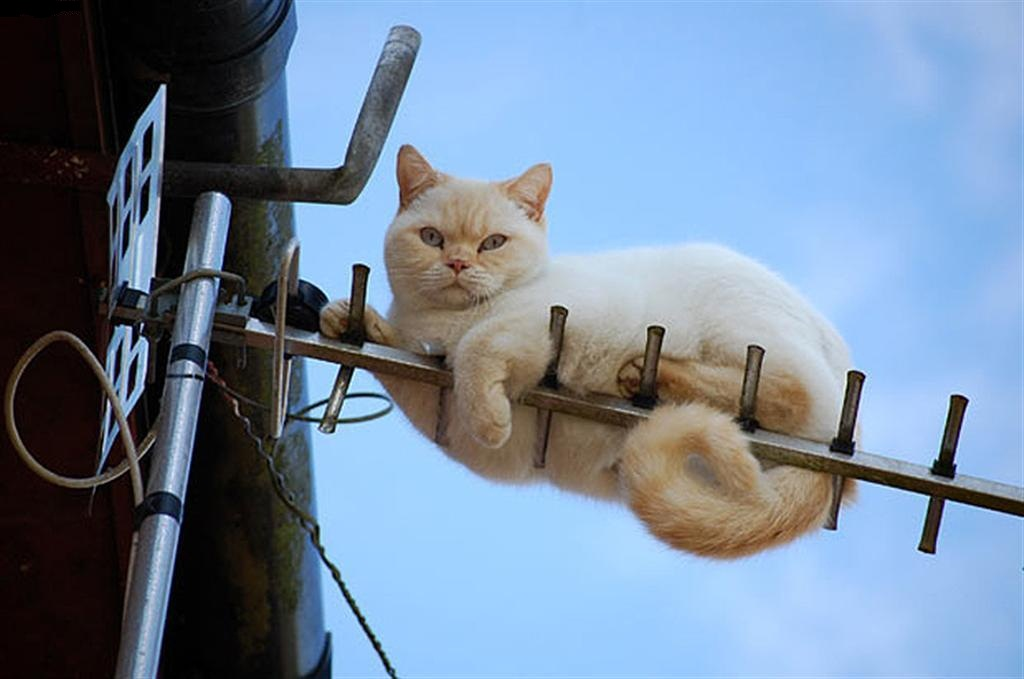
\includegraphics[width=.8\textwidth,height=.75\textheight,keepaspectratio]{e11/cat-antenna.jpg}
      \attribcaption{Cat Antenna}{Jodi Summers}{http://www.socalgreenrealestateblog.com/control-your-homes-energy-use-with-these-apps/cat-antenna/}{}
    \end{figure}
  \end{center}
\end{frame}

\begin{frame}
  \frametitle{Strom und Spannungsverteilung}
  \begin{itemize}
    \item Antennenlänge: $2\cdot\frac{\lambda}{4}$ Strahler
    \item Stromknoten und Spannungsbauch an den Enden (unendlich großer Widerstand)
    \item Spannungsknoten und Strombauch in der Mitte (fast $0 \Omega$ Widerstand)
  \end{itemize}
  \begin{center}
    \begin{figure}
      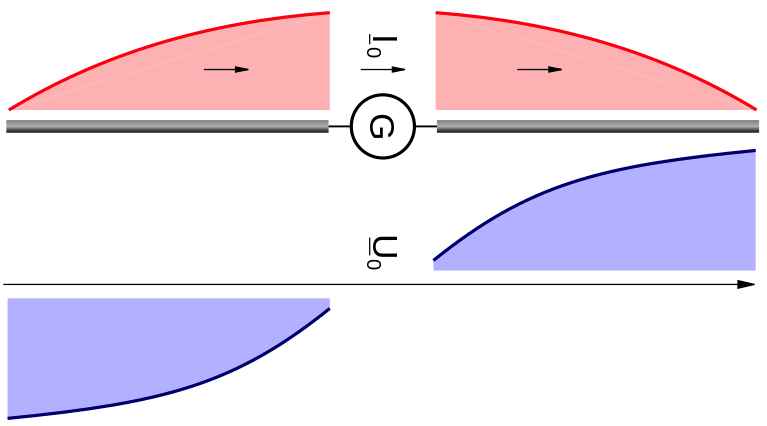
\includegraphics[width=0.85\textwidth,height=.5\textheight,keepaspectratio]{e11/DipolUI.png}
      \attribcaption{Strom- (rot) und Spannungsverlauf (blau) entlang der Stäbe eines Halbwellendipols}{Averse in Zusammenarbeit mit Ulfbastel}{https://commons.wikimedia.org/wiki/File:Lineare_antennen.svg}{\ccbysa}
    \end{figure}
  \end{center}
\end{frame}

\begin{frame}
  \frametitle{Fußpunktwiderstand}
  \begin{center}
    \begin{itemize}
      \item Fußpunktwiderstand/Impedanz/Speisewiderstand
      \item Beim Dipol im Freien Raum: $70 \Omega$
      \item Je nach Dipolhöhe zwischen $40 \Omega$ und $80 \Omega$
      \item Bei $0,15 \lambda$ Höhe $50 \Omega$ Speisewiderstand
    \end{itemize}
  \end{center}
\end{frame}

%\begin{frame}
%    \frametitle{Prüfungsfrage}
%    \begin{center}
%    \begin{tabular}{l||l}\hline
%        TH206 & Ein Halbwellendipol wird auf der  \\
%         " "  & Grundfrequenz in der Mitte \\ \hline\hline
%         A & spannungsgespeist.\\\hline
%         B & stromgespeist. \\\hline
%         C & endgespeist. \\ \hline
%         D & parallel gespeist.\\\hline
%    \end{tabular}
%  \end{center}
%\end{frame}

%\begin{frame}
%    \frametitle{Prüfungsfrage}
%
%    \begin{center}
%    \begin{tabular}{l||l}\hline
%        TH206 & Ein Halbwellendipol wird auf der  \\
%         " "  & Grundfrequenz in der Mitte \\ \hline\hline
%         " " & spannungsgespeist.\\\hline
%         X & stromgespeist. \\\hline
%         " " & endgespeist. \\ \hline
%         " " & parallel gespeist.\\\hline
%    \end{tabular}
%        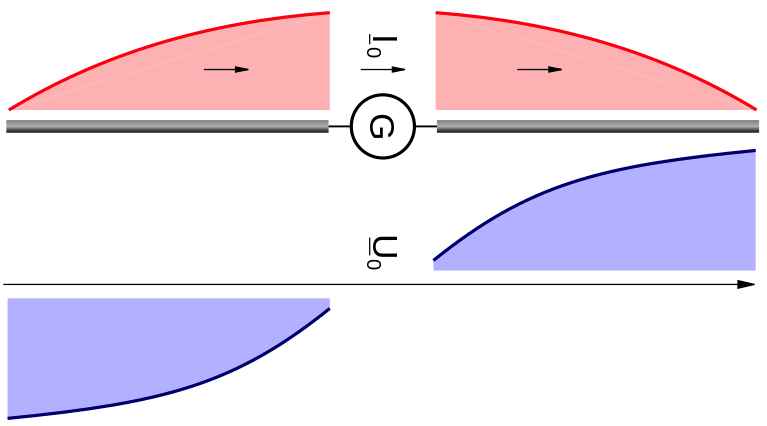
\includegraphics[width=0.85\textwidth]{e11/DipolUI.png}
%        \footnote{\tiny \url{https://commons.wikimedia.org/wiki/%File:Lineare_antennen.svg}}
%  \end{center}
%\end{frame}


\begin{frame}
  \frametitle{Fußpunktwiderstand}
  \begin{center}
    \begin{itemize}
      \item Erwünschter Widerstand: Real $50 \Omega$ Imaginär $O \Omega$
      \item SWR-Meter (Standing wave Ratio) möglichst 1:1
    \end{itemize}
  \end{center}
\end{frame}

\begin{frame}
  \frametitle{SWR}
  \begin{center}
    \begin{itemize}
      \item Aussage über Verhältnis Widerstand am Kabelende zu Widerstand an der Antenne
      \item Informationen darüber wie viel Leistung an die Antenne abgegeben wird
      \item Nicht an die Antenne gegebene Leistung wird zurück in die Endstufe reflektiert
      \item Keine Aussage über Abstrahleigenschaften der Antenne ($50 \Omega$ R ist perfekt)
      \item Typische Werte für eine reale Antenne im WLAN-Bereich liegen etwa bei 2:1 bis 2,5:1.
      \item Für rad1o werden Antennen benötigt mit SWR besser als 2:1
    \end{itemize}
  \end{center}
\end{frame}

\begin{frame}
  \frametitle{Schwingkreis}
  \begin{center}
    \begin{figure}
      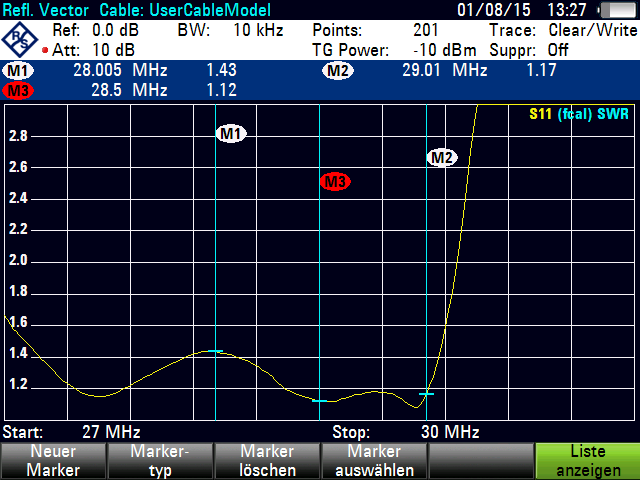
\includegraphics[width=.7\textwidth,height=.75\textheight,keepaspectratio]{e11/Measurement0010.png}
      \caption{Messung einer selbstgebauten Yagi für $10m$ bei DK\O TU}
    \end{figure}
  \end{center}
\end{frame}


\section*{Richtdiagramm}

\begin{frame}
  \frametitle{Richtdiagramm Dipol}
  \begin{center}
    \begin{figure}
      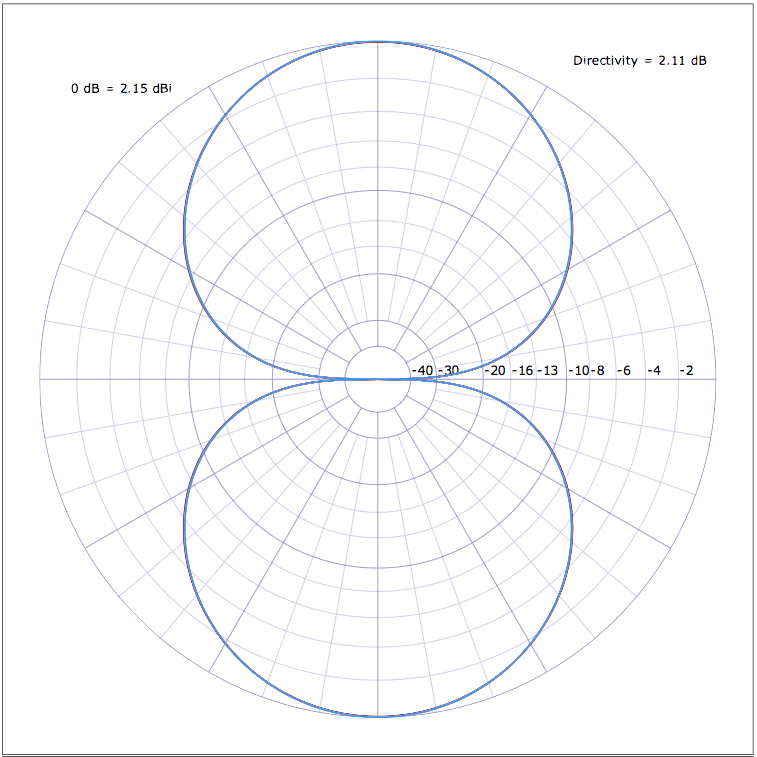
\includegraphics[width=0.6\textwidth,height=.75\textheight,keepaspectratio]{e11/Richt-Dipol.png}
      \caption{DB4UM Programm: cocoaNec 2.0}
    \end{figure}
  \end{center}
\end{frame}

\section*{Gewinn}

\begin{frame}
  \frametitle{ERP und EIRP}
  \begin{itemize}
    \item ERP
      \begin{itemize}
        \item Effective Radiated Power
        \item Bezug auf Dipol
        \item $P_{ERP} = G_{Dipol} \cdot (P_{Sender} - P_{Verlust})$
      \end{itemize}
    \item EIRP
      \begin{itemize}
        \item Equivalent Isotropically Radiated Power
        \item Bezug auf Isotropstrahler
        \item $dB_{ERP} = 2,15 + dB_{EIRP}$
        \item $P_{EIRP} = 1,64 \cdot P_{ERP}$
      \end{itemize}
  \end{itemize}
\end{frame}

\begin{frame}
  \frametitle{Isotropstrahler}
  \begin{center}
    \begin{figure}
      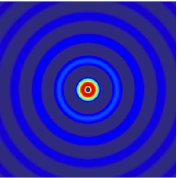
\includegraphics[width=0.65\textwidth,height=.75\textheight,keepaspectratio]{e11/Spherical_wave2.png}
      \attribcaption{Sphärische Welle}{Oleg Alexandrov}{https://commons.wikimedia.org/wiki/File:Spherical_wave2.gif}{\ccpd}
    \end{figure}
  \end{center}
\end{frame}

\section*{Multiband}

\begin{frame}
  \frametitle{Multiband Dipol}
  Gewinn: 2,15dBi
  \begin{center}
    \begin{figure}
      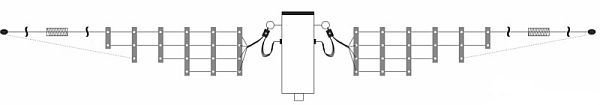
\includegraphics[width=0.9\textwidth,height=.75\textheight,keepaspectratio]{e11/Multiband.jpg}
      \caption{Antenne EA-1015204080 von EAntenna}
    \end{figure}
  \end{center}
\end{frame}

\begin{frame}
  \frametitle{G5RV}
  \begin{center}
    \begin{figure}
      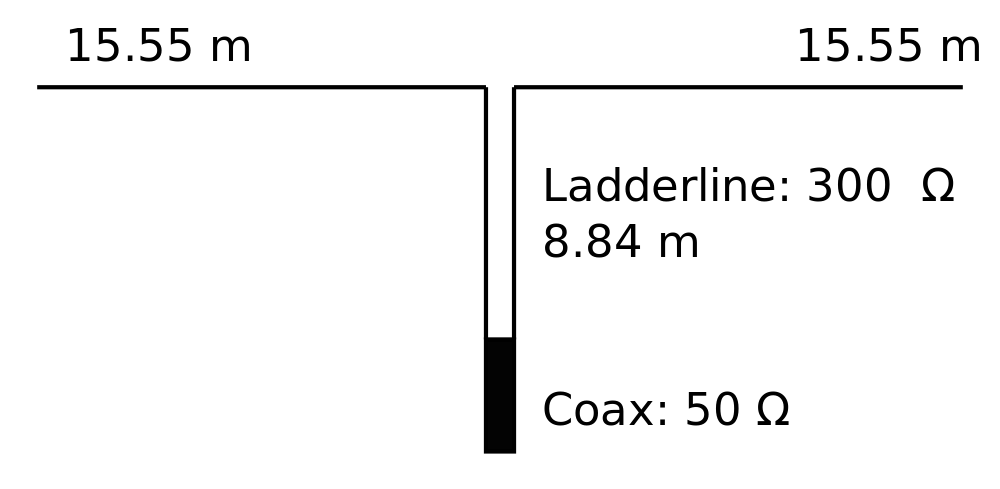
\includegraphics[width=0.9\textwidth,height=.75\textheight,keepaspectratio]{e11/G5RV_Antenna.png}
      \attribcaption{G5RV Antenne}{Gerolf Ziegenhain}{https://commons.wikimedia.org/wiki/File:G5RV_Antenna.svg}{\ccbysa}
    \end{figure}
  \end{center}
\end{frame}


\section*{Yagi-Uda}

\begin{frame}
  \frametitle{Yagi-Uda}
  $5dBi$-$30dBi$
  \begin{center}
    \begin{figure}
      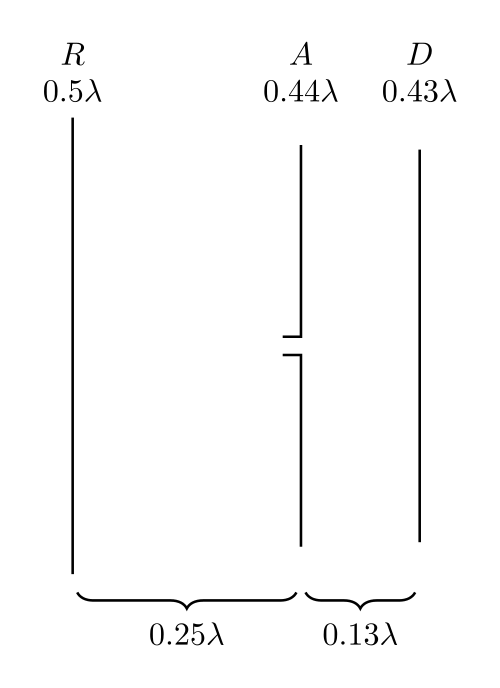
\includegraphics[width=0.36\textwidth,height=.7\textheight,keepaspectratio]{e11/Yagi_3_element.png}
      \attribcaption{3 Element Yagi Antenne}{Sankeytm}{https://commons.wikimedia.org/wiki/File:Yagi_3_element.svg}{\ccbysa}
    \end{figure}
  \end{center}
\end{frame}


\begin{frame}
  \frametitle{Richtdiagramm Yagi}
  \begin{center}
    \begin{figure}
      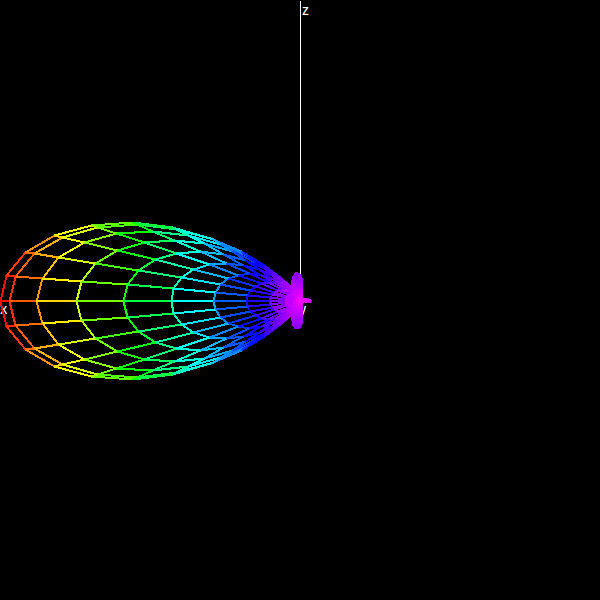
\includegraphics[width=0.55\textwidth,height=.75\textheight,keepaspectratio]{e11/yagi_gain.png}
      \caption{DK\O TU 10m Yagi 28.1 MHz von DL2JAS Programm: EZNEC}
    \end{figure}
  \end{center}
\end{frame}

\begin{frame}
  \frametitle{Yagi - Richtung erkennen}
  \begin{center}
    \begin{figure}
      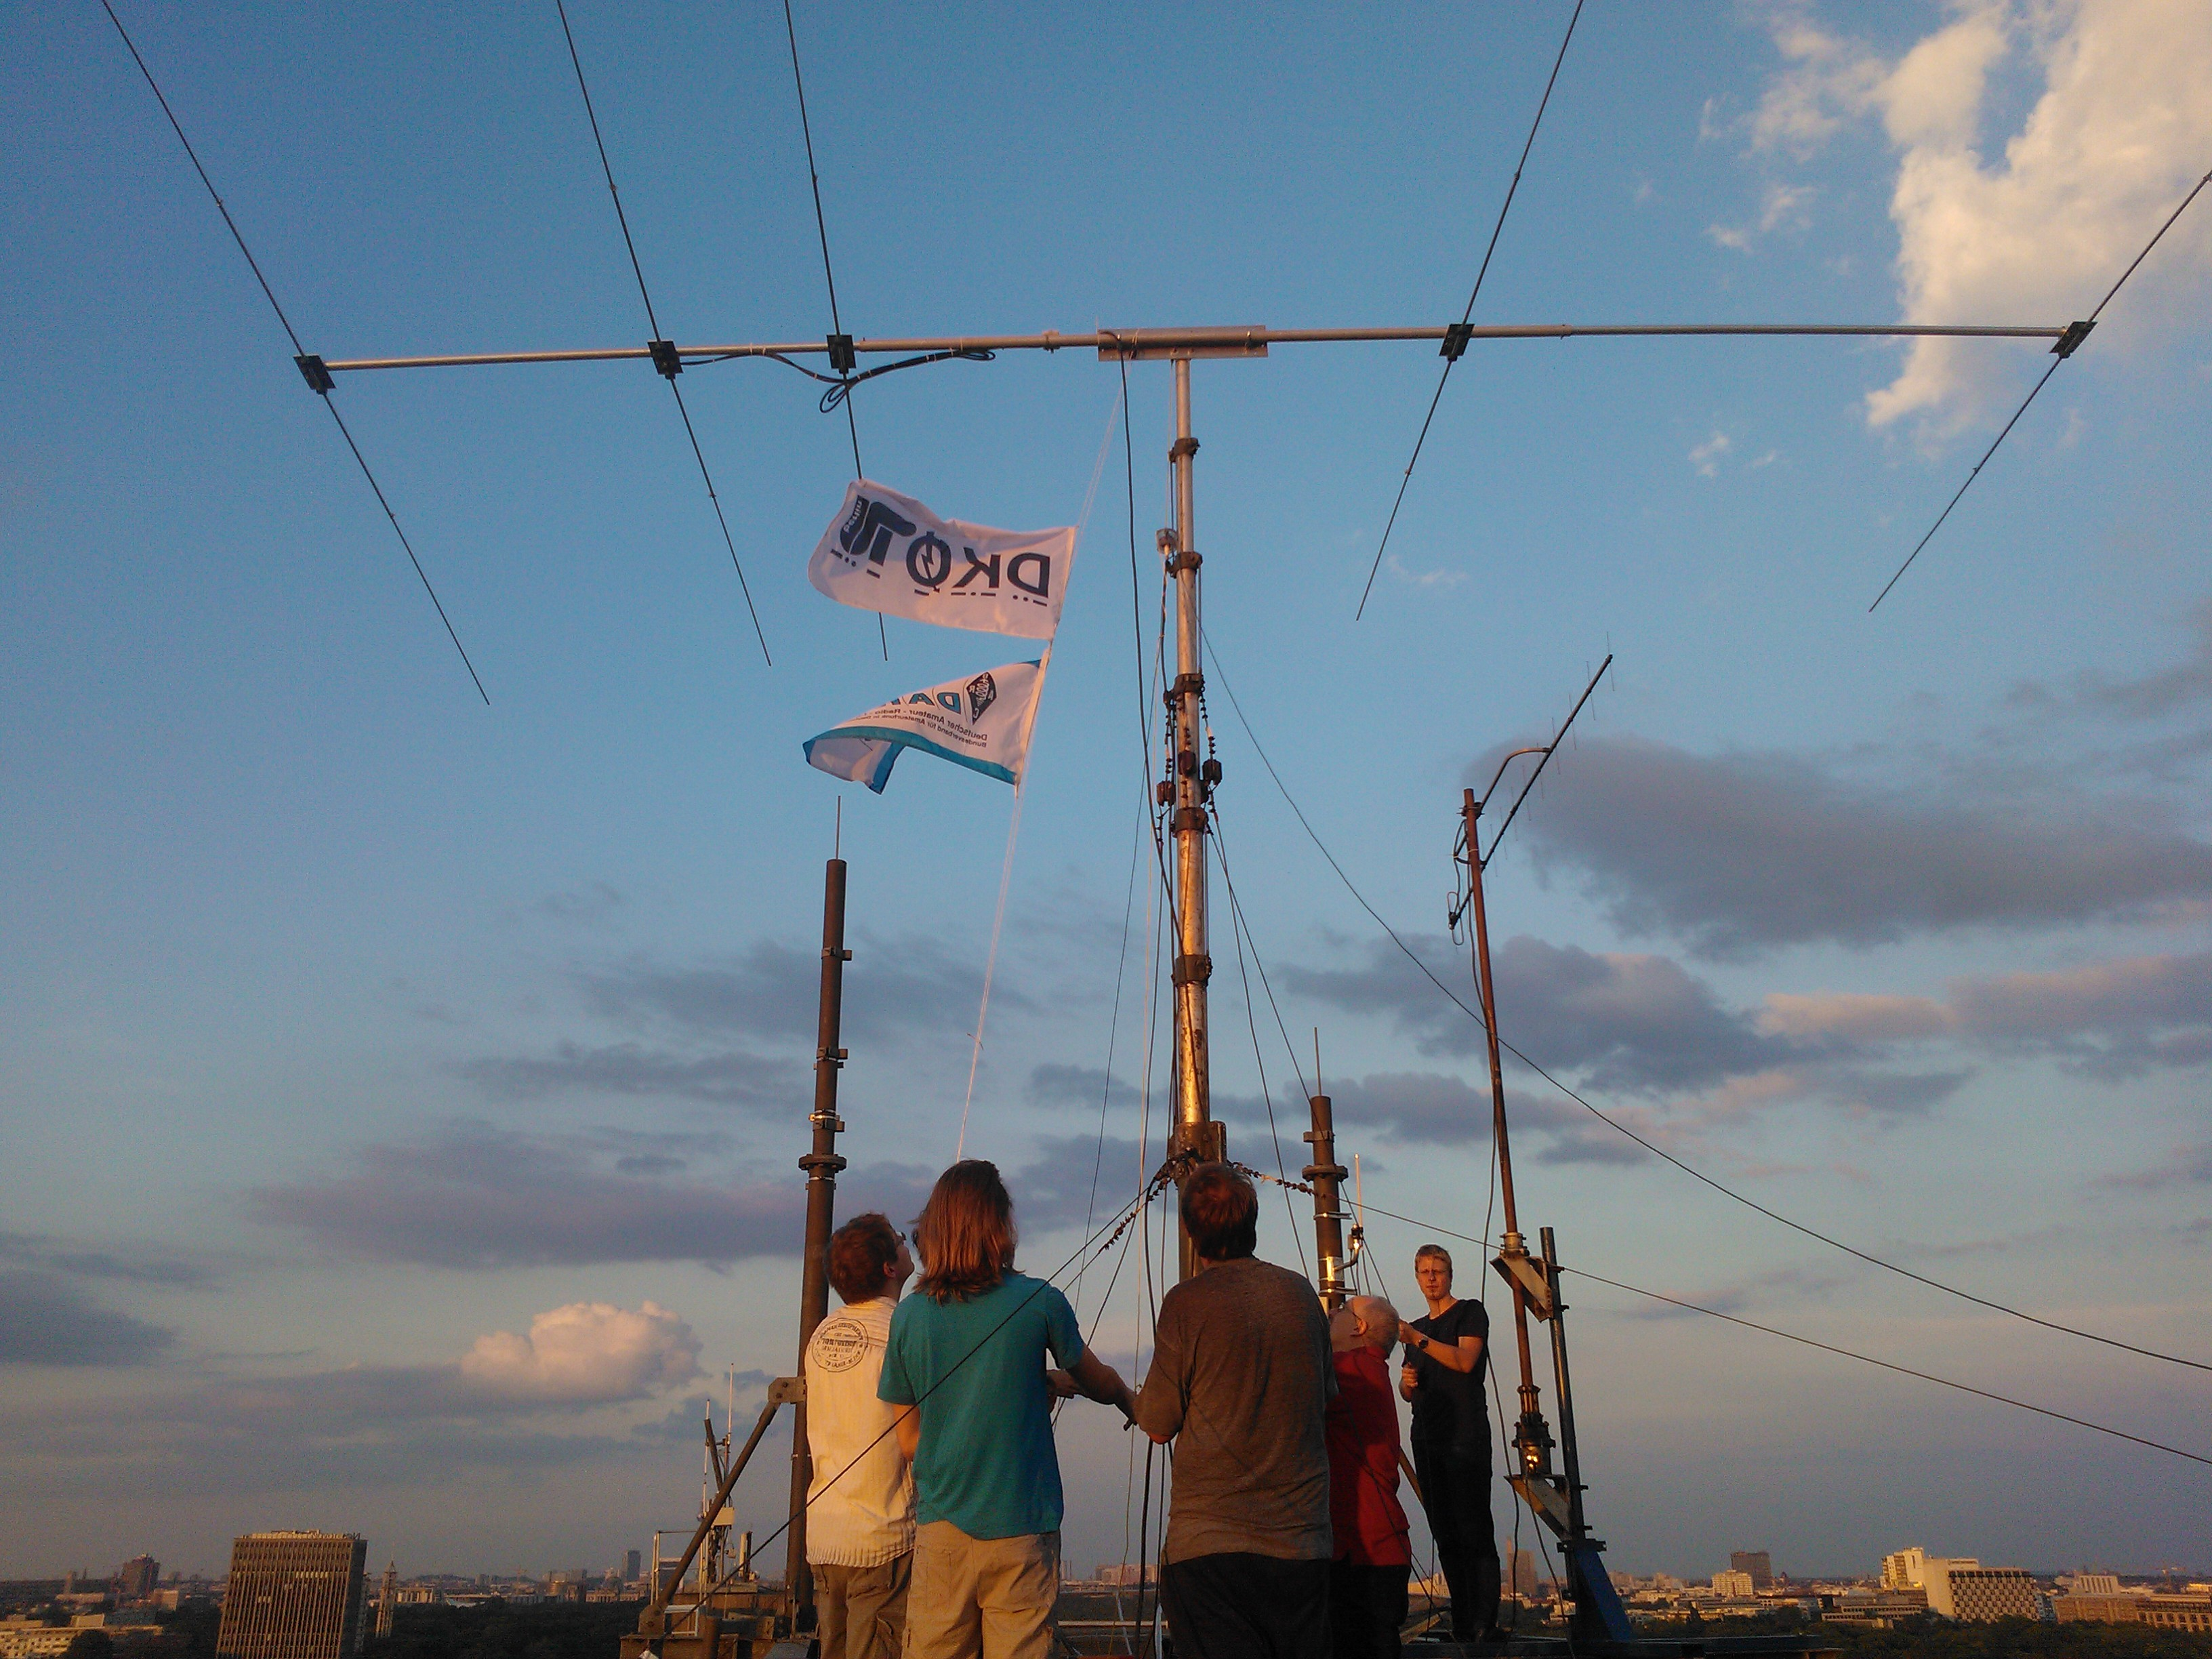
\includegraphics[width=.75\textwidth,height=.75\textheight,keepaspectratio]{e11/yagi.jpg}
      \caption{10M Yagi bei DK\O TU von DK9GD}
    \end{figure}
  \end{center}
\end{frame}


\section*{Groundplane}

\begin{frame}
  \frametitle{Groundplane}
  $2.15dBi$ - Jeder Draht $\frac{\lambda}{4}$
  \begin{center}
    \begin{figure}
      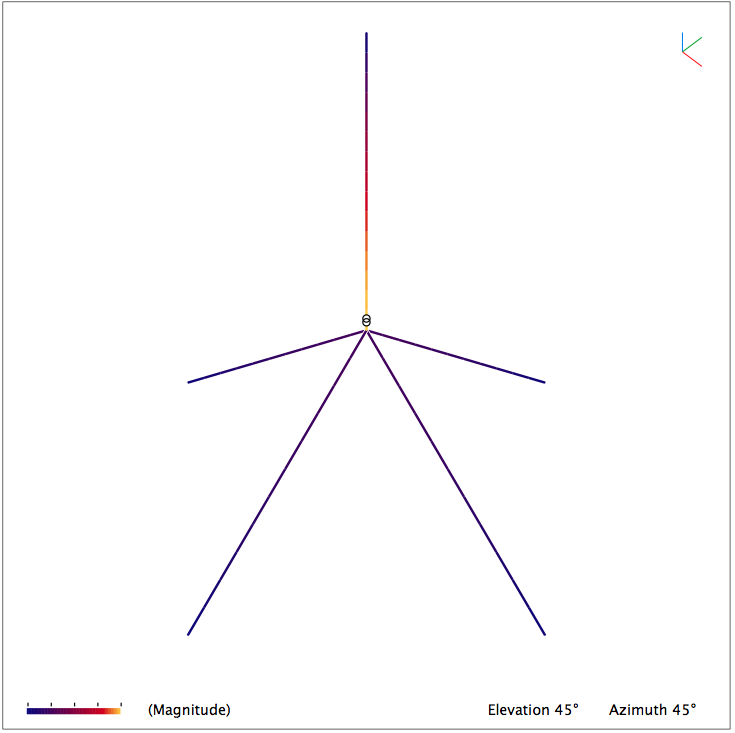
\includegraphics[width=0.6\textwidth,height=.7\textheight,keepaspectratio]{e11/GP-DB4UM.png}
      \caption{DB4UM mit cocoaNec 2.0}
    \end{figure}
  \end{center}
\end{frame}

\begin{frame}
  \frametitle{Spiegelladung}
  \begin{center}
    \begin{figure}
      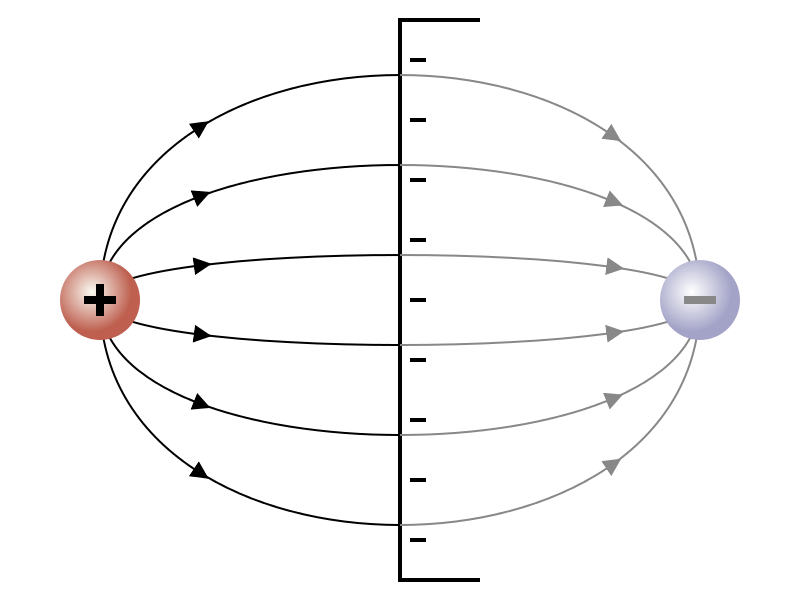
\includegraphics[width=0.7\textwidth,height=.75\textheight,keepaspectratio]{e11/Spiegelladung.png}
      \attribcaption{Spiegelladung einer positiven Ladung an einer Metallfläche}{Paeng}{https://de.wikipedia.org/wiki/Datei:Spiegelladung.svg}{\ccbysa}
    \end{figure}
  \end{center}
\end{frame}

\begin{frame}
  \frametitle{Spiegelladung}
  \begin{center}
    \begin{figure}
      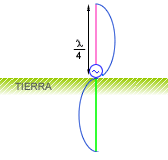
\includegraphics[width=0.55\textwidth,height=.75\textheight,keepaspectratio]{e11/Antena_marconi501.png}
      \attribcaption{Marconi Antenne}{n/a}{https://commons.wikimedia.org/wiki/File:Antena_marconi501.png}{\ccpd}
    \end{figure}
  \end{center}
\end{frame}

\begin{frame}
  \frametitle{Magnetfuss-Antenne}
  \begin{center}
    \begin{figure}
      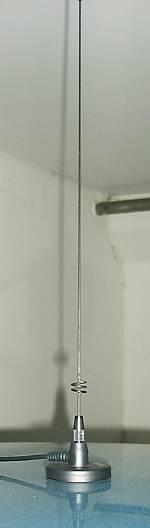
\includegraphics[height=0.8\textheight,height=.75\textheight,keepaspectratio]{e11/magnetfuss.jpg}
      \caption{Magnetfuss-Antenne}
    \end{figure}
  \end{center}
\end{frame}

\section*{Magnetic Loop}

\begin{frame}
  \frametitle{Magnetic Loop}
  \begin{center}
    \begin{figure}
      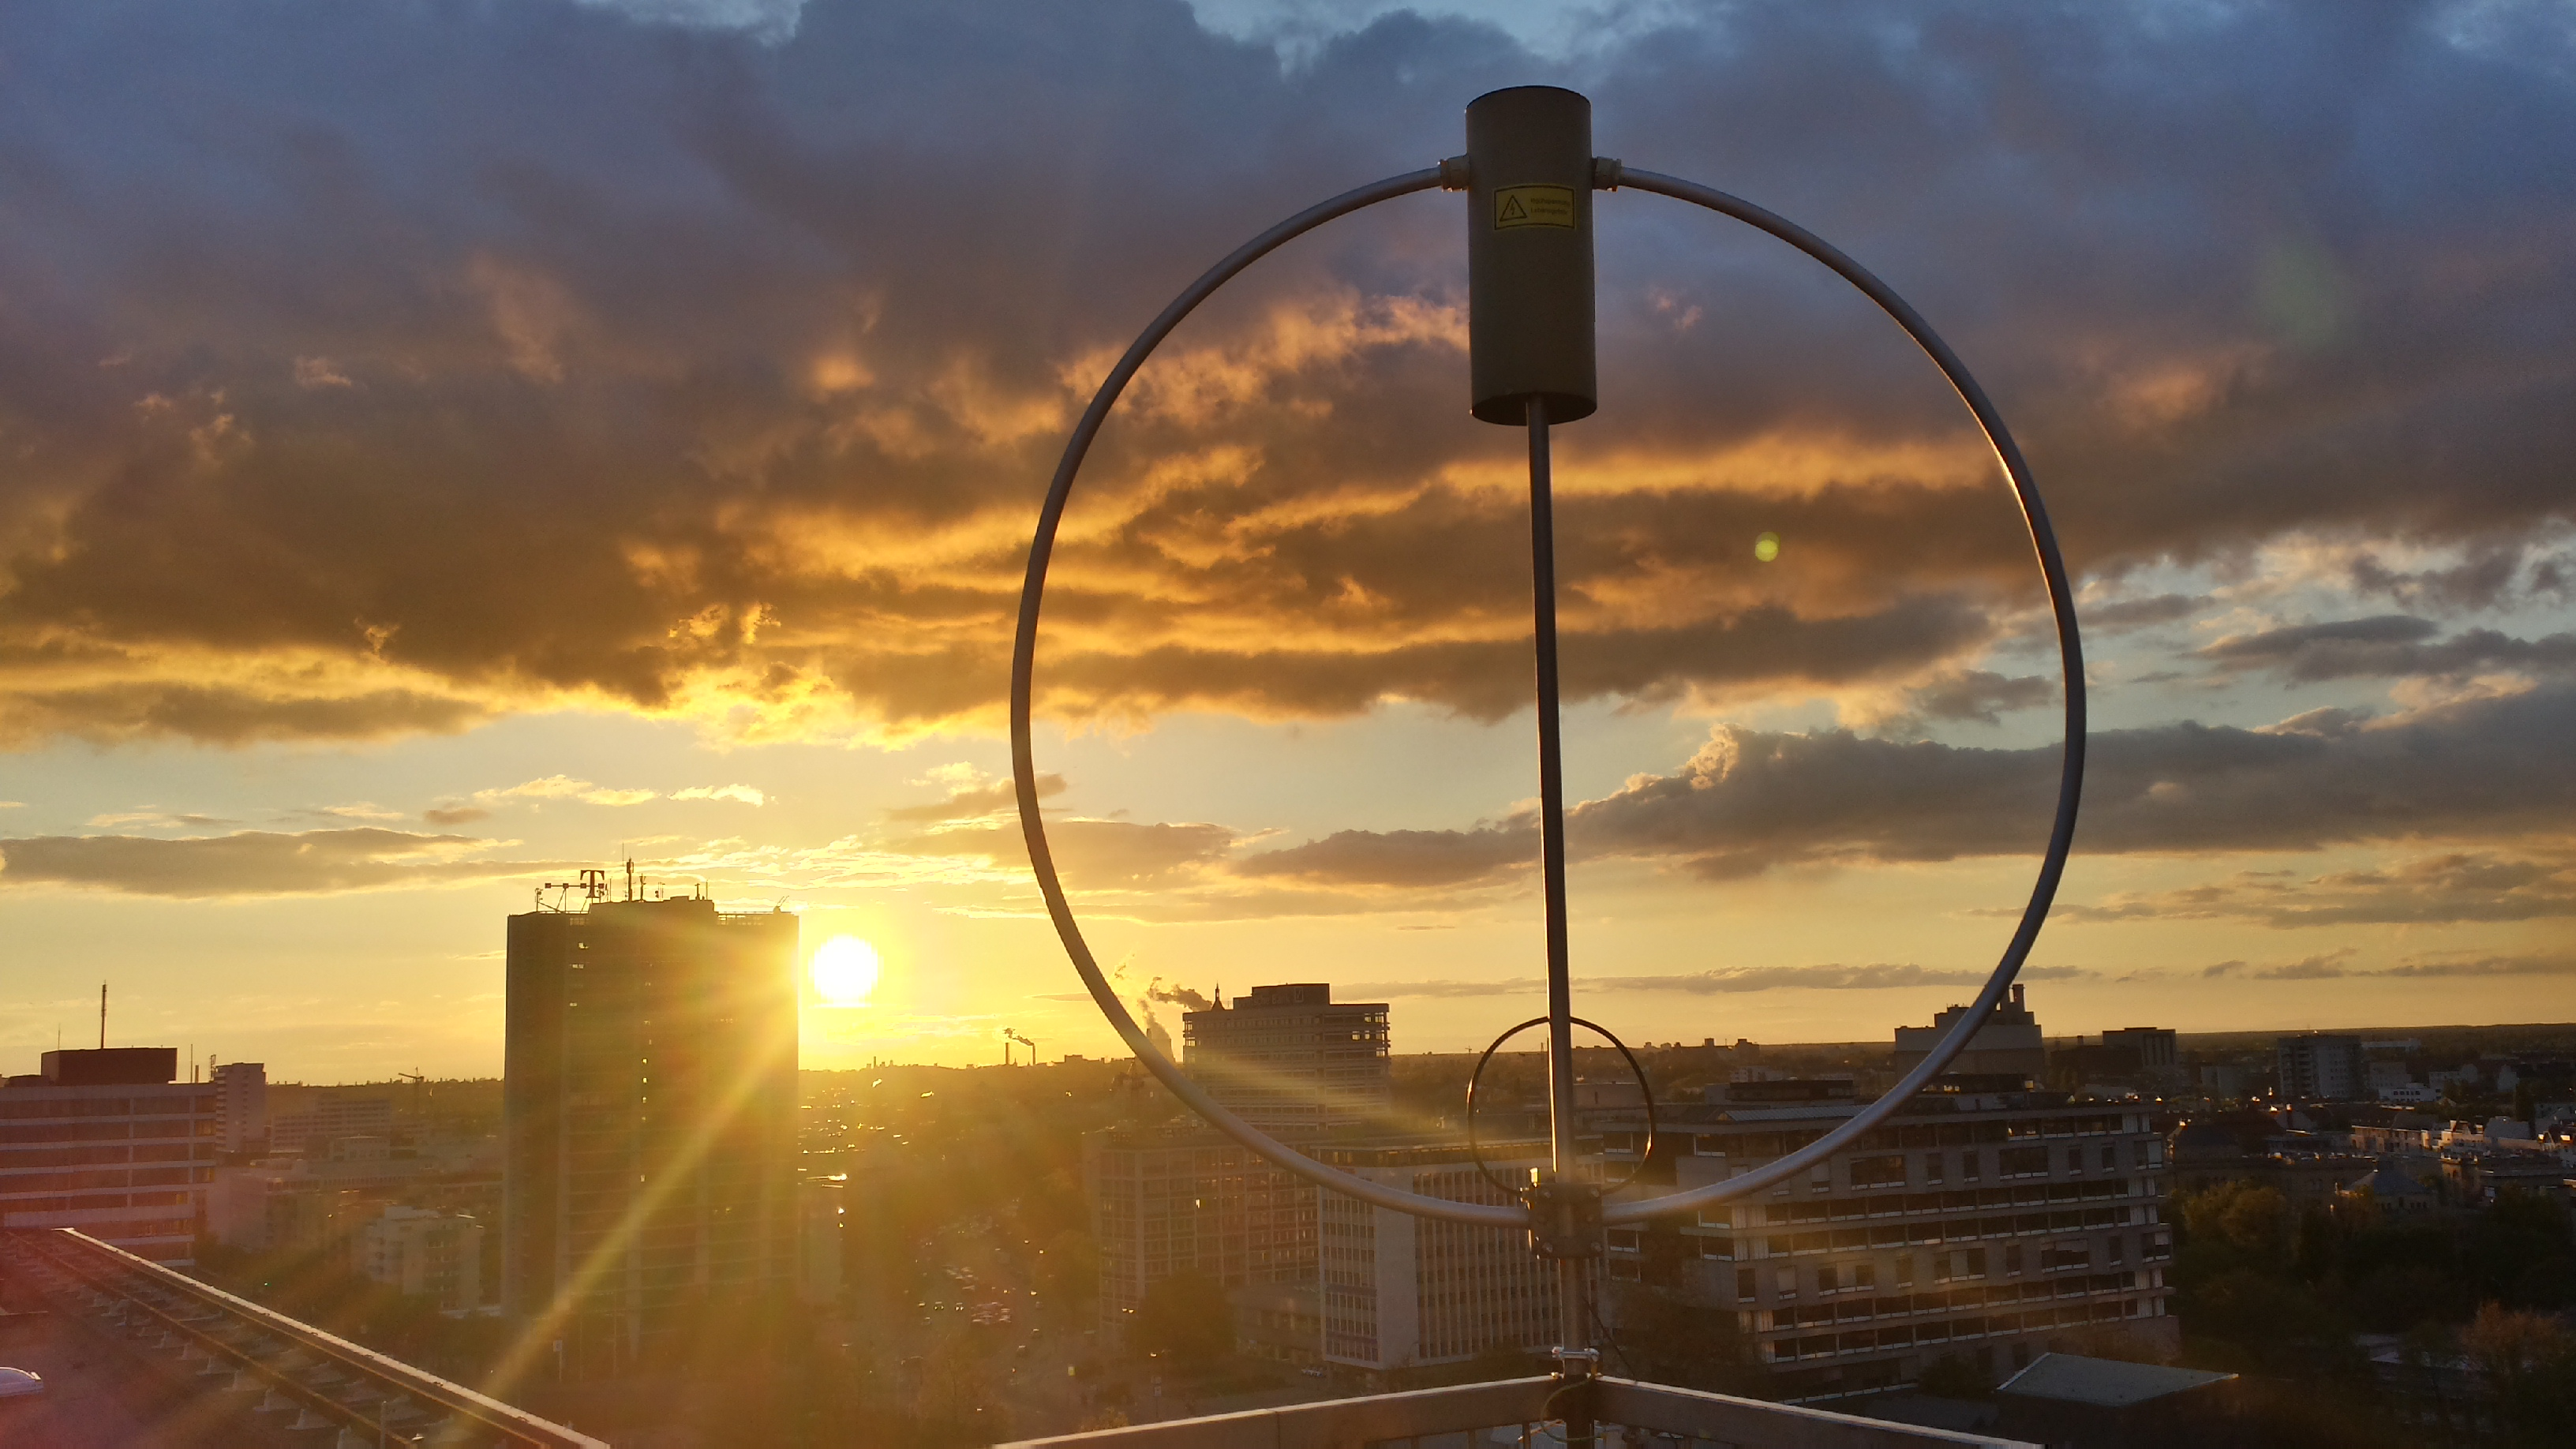
\includegraphics[width=0.89\textwidth,height=.75\textheight,keepaspectratio]{e11/Magloop.jpg}
      \caption{Magloop bei DK\O TU von DB4UM}
    \end{figure}
  \end{center}
\end{frame}

\section*{Portabelfunk}

\begin{frame}
  \frametitle{Portabel Kurzwellenfunk}
  \begin{center}
    \begin{figure}
      \includegraphics[height=.83\textheight,height=.75\textheight,keepaspectratio]{e11/portabelFunk.png}
      \caption{C-Pole Antenne für 20m im Mauerpark \#berlinUrbanHamRadio}
    \end{figure}
  \end{center}
\end{frame}

\section*{Polarisierung}

\begin{frame}
  \frametitle{Polarisierung}
  \begin{itemize}
    \item Welche Antennen sind vertikal, welche horizontal polarisiert?
    \item Wie ist die Antenne unten polarisiert?
  \end{itemize}
  \begin{center}
    \begin{figure}
      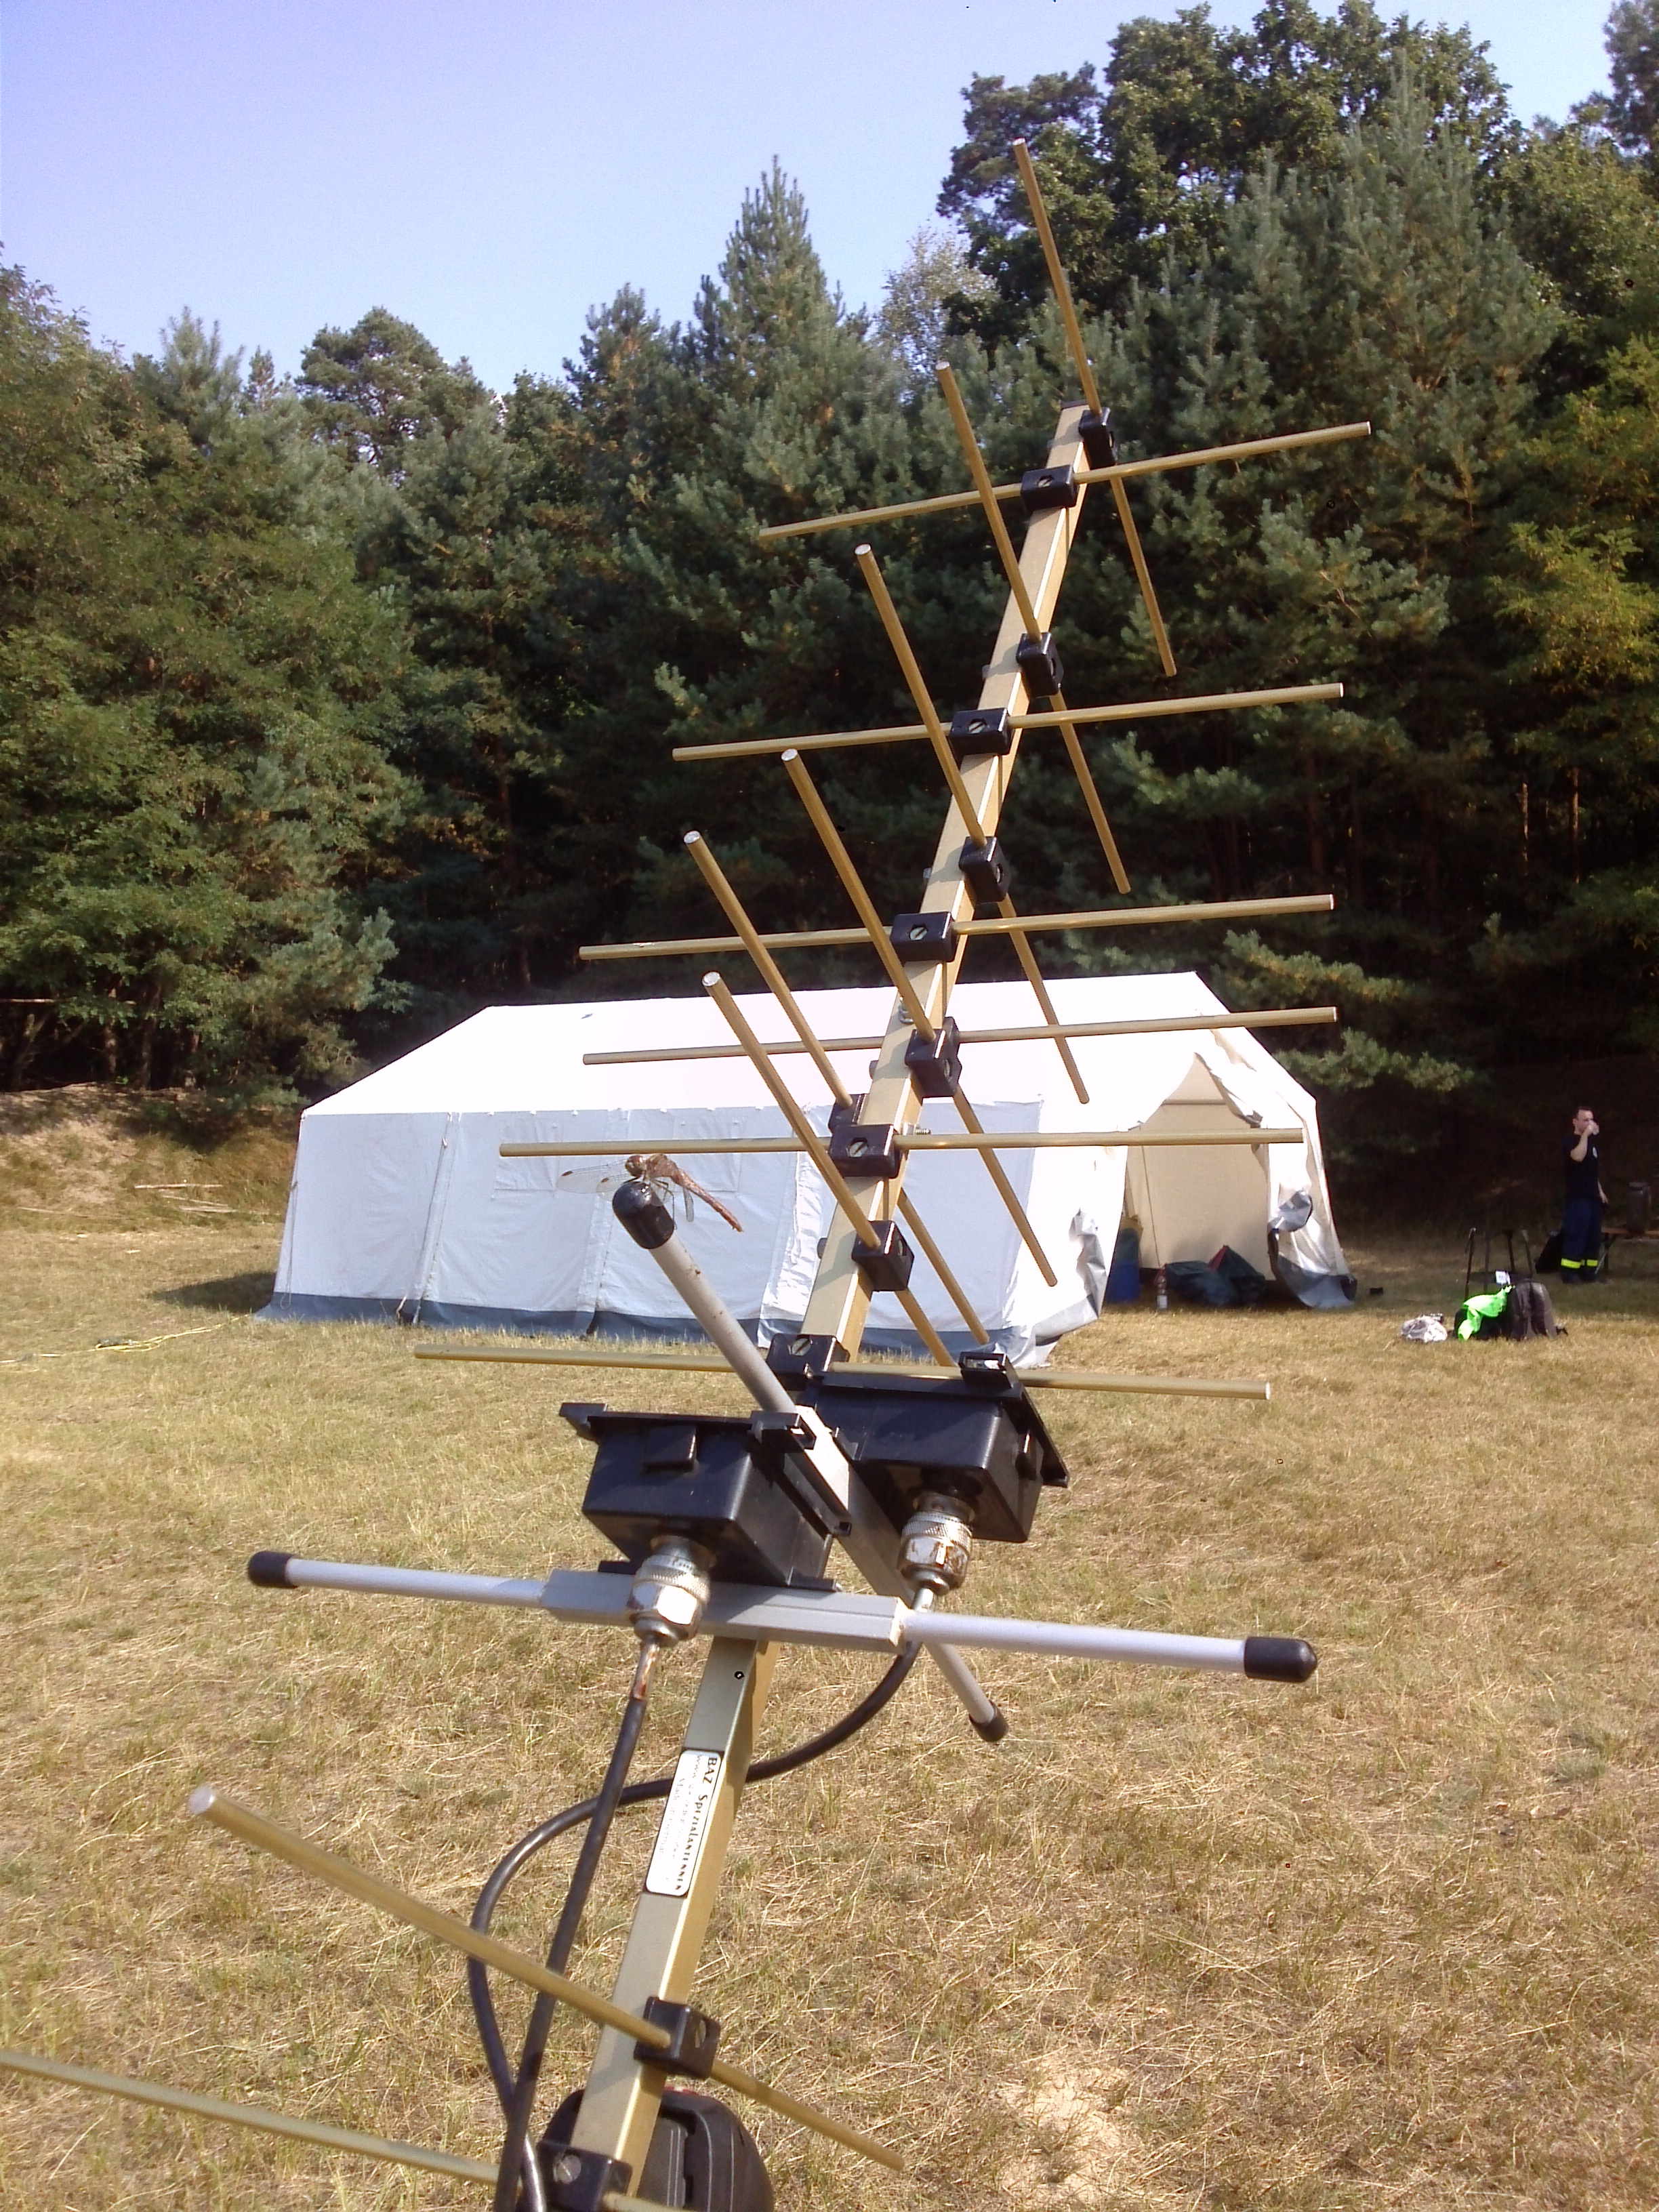
\includegraphics[width=.3\textwidth,height=.75\textheight,keepaspectratio]{e11/kreutzYagi.jpg}
      \caption{DK\O TU Fieldday 2014 von DL7BUR}
    \end{figure}
  \end{center}
\end{frame}

%\begin{frame}
%    \frametitle{Jetzt Ihr}
%    \begin{center}  Baut, messt und benutzt eure selbstgebauten Antennen
%        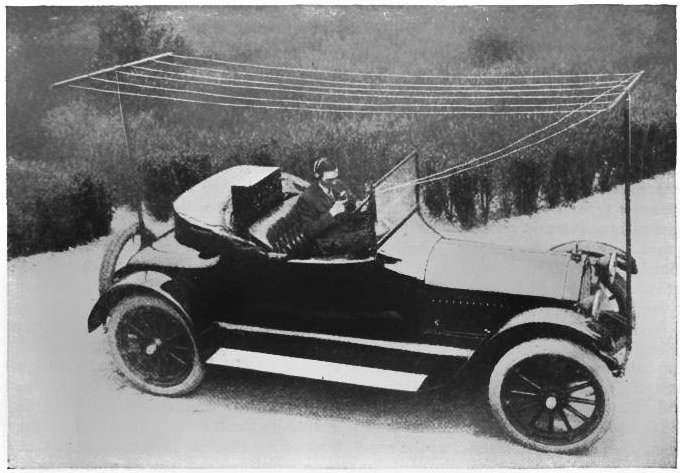
\includegraphics[width=1\textwidth]{e11/hamPro.jpg}
% \end{center}
%\end{frame}

%\begin{frame}
%    \frametitle{Kontakt}
%     \begin{itemize}
%  \item Twitter: [at]b4um oder [at]dk0tu%
%  \item baum AT campus.tu-berlin.de
%  \item GSM: B4UM
%  \item Amateur Radio Dorf
%    \end{itemize}
%\end{frame}


\section*{Referenzen}

\begin{frame}
  \frametitle{Referenzen/Links}

  \footnotesize
  \begin{itemize}
    \item Moltrecht E 11: \\
      \url{https://www.darc.de/der-club/referate/ajw/lehrgang-te/e11/}
    \item Strahlungsdiagramm (Youtube): \\
      \url{https://www.youtube.com/watch?v=gBqqp7rnZ64}
  \end{itemize}

\end{frame}


% Hier könnte noch eine Kontaktfolie stehen

\end{document}

